\documentclass[12 pts,spanish]{article}
\oddsidemargin 0in
\textwidth 6.75in
\topmargin 0in
\textheight 8.5in
\parindent 0em
\parskip 1ex

\usepackage{graphicx}

\begin{document}
\title{Proyecto de Programacion I  Moogle!\\Universidad de la Habana \\ Facultad de Matematica y Computacion}
\author{Daniela de la Caridad Guerrero Alvarez}
\maketitle


\begin{figure}[ht]
    \centering
    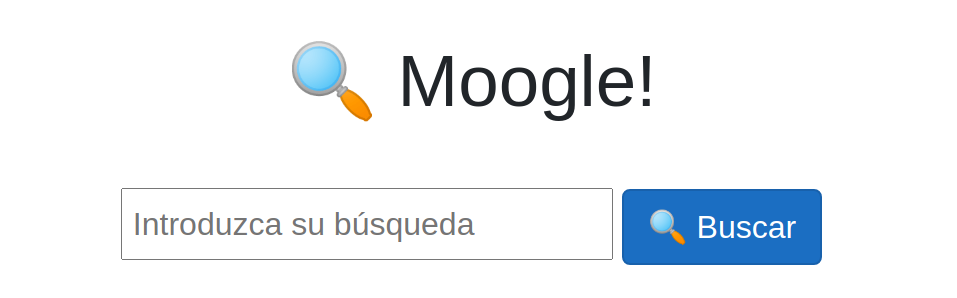
\includegraphics[width=5in]{moogle.png}
    \caption{}
    \label{fig:Moogle}
\end{figure}
\section{Introduccion}
Este proyecto consiste en la realización de una aplicación cuyo propósito es realizar búsquedas de forma inteligente de un texto especifico en un conjunto de documentos.
Es una aplicación web, desarrollada con tecnología .NET Core 6.0, específicamente usando Blazor como *framework* web para la interfaz gráfica, y en el lenguaje C\#.

\section{Estructura del Proyecto}
En la realización del proyecto se utilizo el Modelo de Recuperacion de Informacion Vectorial ,el cual se basa en el grado de similaridad de la consulta dada por el usuario con respecto a los documentos de la colección cuyos términos fueron ponderados mediante TF-IDF(Term Frequency – Inverse Document Frequency).\\ 
\begin{figure}[h]
    \center
    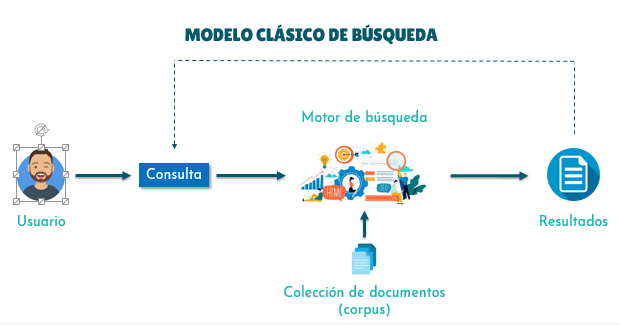
\includegraphics[width=6in]{estructura.png}
    \caption{}
    \label{fig:Estructura del Proyecto}
\end{figure}

En el proyecto se definieron otras clases para mayor organizacion y legibilidad del codigo ,las cuales son:
\begin{enumerate}
    \item La clase Initialize en la cual se hace todo el proceso de cargar,leer,normalizar los documentos y clacular el TF-IDF de los documentos.En esta clase tenemos los metodos:
    \begin{enumerate}
        \item Read:Este metodo recibe los documentos y los normaliza.
        \item FillFilesWords: Este metodo llena un diccionario con las palabras y su Tf.\\Para calcular el Tf se utiliza la siguiente formula :
        \begin{equation}
            Tf = \frac{freq_{i,j}}{max_{l}freq_{ l,j}}
        \end{equation}
         
        \item FillIdf :Este metodo calcula el idf de todas las palabras de los documentos y crea un diccionario con las palabras y su valor de idf \\Para calcular el idf utiliza la siguiente formula :
        \begin{equation}
            Idf=\log{\frac{N}{n_{i}}}
        \end{equation}

        \item DocWeigth:Este metodo recibe el diccionario con las palabras con su Tf y el diccionario con el idf de las palabras y los multiplica con la siguiente formula:
        \begin{equation}
            W_{i,j}=\frac{tf_{i,j}}{idf_{i}}
        \end{equation} 

    \end{enumerate}
    \item La clase ProcessQuery la cual es la encargada de normalizar la query y calcular el Tf-Idf de la misma.En esta clase se encuentran los metodos :
    \begin{enumerate}
        \item Normalize : El cual recibe la busqueda del usuario, la normaliza y la divide en palabras.
        
        \item FillQueryWordsTf :Este metodo recibe un string query y llama al metodo Normalize.Luego crea un  diccionario con la forma < palabras de la query,tf de las palabras de la query > y retorna ese diccionario.
        
        \item TfIdfQuery : Este metodo recibe el diccionario con las palabras de la query con su Tf y el diccionario con todas las palabras de los documentos y su Idf y devuelve un diccionario con las palabras de la query y su Tf-Idf.
        
    \end{enumerate}
    \item La clase FIllScore es la encargada de calcular la similitud entre el vector documento y la consulta utilizando la siguiente formula :
    \begin{equation}
     similitud(d_{j},q) = \frac{\sum_{i=1}^{n} W_{i,j} x  W_{iq}}{\sqrt{\sum_{i=1}^{n} W_{i,j}^2}  x  \sqrt{\sum_{i=1}^{n} W_{i,q}^2}}
    \end{equation} 
    
\end {enumerate}

\section{Resultados de la Busqueda}
Despues de realizar todos los procesos antes descritos la aplicacion muestra como resultado de la busqueda del usuario , en el caso en que aparezca especificamente alguna palabra de la consulta , tres documentos donde se encuntra alguna de las palabras y un fragmento de los documentos donde aparezca al menos una palabra de la query .
\end{document}